\documentclass{article}
\usepackage{url}

\usepackage{cite,enumitem,amsmath, amsfonts, amssymb}
\usepackage{epsfig,subfigure}
\usepackage{comment}
\usepackage{array}


\newcommand\dueDate{Tuesday, Nov.~10, 2020 (11am)}

\input assignment_utils
\usepackage{listings}


\begin{document}
\createHomework{2}




%%%%%%%%%%%%%%%%%%%%%%%%%%%%%%%%%%%%%%%%%%%%%%%%%%%%%%%%%%%%
\begin{problem}{Mutual coherence}{40}

For an arbitrary pair of orthonormal bases $\bm{\Psi}=[\bm{\psi}_1, \cdots, \bm{\psi}_n] \in \mathbb{R}^{n\times n}$ and $\bm{\Phi}=[\bm{\phi}_1,\cdots,\bm{\phi}_n] \in \mathbb{R}^{n\times n}$, the mutual coherence $\mu(\bm{\Psi}, \bm{\Phi})$ of these two bases is defined by 
\begin{equation}
  \mu(\bm{\Psi}, \bm{\Phi}) = \max_{1\leq i,j\leq n} \left| \bm{\psi}_i^{\top} \bm{\phi}_j  \right| \label{eq:mutual-coherence}
\end{equation}


\newpart{0}
Show that 
\[
  \frac{1}{\sqrt{n}} \leq \mu(\bm{\Psi}, \bm{\Phi}) \leq 1.
\]

\solution{
By definition, 
\begin{align}
  \mu(\bm{\Psi}, \bm{\Phi}) & = \max_{1\leq i,j\leq n} \left| \bm{\psi}_i^{\top} \bm{\phi}_j  \right| 
			    \geq  \sqrt{ \frac{1}{n^2} \sum_{1\leq i,j\leq n} \left| \bm{\psi}_i^{\top} \bm{\phi}_j  \right|^2 } \\
    & = \sqrt{ \frac{1}{n^2}  \| \bm{\Psi}^{\top} \bm{\Phi} \|_{\mathrm{F}}^2  }. 
\end{align}

Recognizing that $\| \bm{\Psi}^{\top} \bm{\Phi} \|_{\mathrm{F}}^2 = \mathrm{tr}(\bm{\Psi}^{\top} \bm{\Phi}  \bm{\Phi}^{\top} \bm{\Psi}) = n$, we obtain $ \mu(\bm{\Psi}, \bm{\Phi}) \geq \frac{1}{\sqrt{n}}$.
}

\newpart{0}
Let $\bm{\Psi} = \bm{I}$, and suppose that $\bm{\Phi} = [\phi_{i,j}]_{1\leq i,j\leq n}$ is a Gaussian random matrix such that the $\phi_{i,j}$'s are i.i.d.~random variables drawn from $\phi_{i,j} \sim \mathcal{N}(0, 1/n)$.  Can you provide an upper estimate on $\mu(\bm{\Psi}, \bm{\Phi})$ as defined in (\ref{eq:mutual-coherence})?  Since $\bm{\Phi}$ is a random matrix, we expect your answer to be a function $f(n)$ such that $\mathbb{P}\{\mu(\bm{\Psi}, \bm{\Phi}) > f(n)\} \rightarrow 0$ as $n$ scales. 
%How does your estimate compare to the lower bound (\ref{eq:mutual-coherence})?

\vspace{0.5em}
Hint: to simplify analysis, you are allowed to use the  crude approximation $\mathbb{P}\{ |z| > \tau\} \approx  \exp( - \tau^2 /2 )$ for large $\tau >0$, where $z\sim \mathcal{N}(0,1)$.

\solution{
Note that $\bm{\Psi}=[\bm{e}_{1},\cdots,\bm{e}_{n}]$ with $\bm{e}_{i}$
the $i$th standard basis vector. One has
\[
\mu(\bm{\Psi},\bm{\Phi})=\max_{1\leq i,j\leq n}|\langle\bm{e}_{i},\bm{\phi}_{j}|\leq\max_{1\leq i,j\leq n}|\phi_{i,j}|.
\]
This boils down to understanding the maximum magnitude of a set of i.i.d.~Gaussian
variables. For any sufficiently large $\tau>0$,
\begin{eqnarray}
\mathbb{P}\left\{ \max_{1\leq i,j\leq n}|\phi_{i,j}|>\frac{\tau}{\sqrt{n}}\right\}  & \leq & \sum_{1\leq i,j\leq n}\mathbb{P}\left\{ \sqrt{n}|\phi_{i,j}|>\tau\right\} \label{eq:inequality1}\\
 & \approx & n^{2}\exp\left(-\frac{\tau^{2}}{2}\right)\label{eq:inequality2}\\
 & = & \exp\left(2\log n-\frac{\tau^{2}}{2}\right),
\end{eqnarray}
 where (\ref{eq:inequality1}) follows from the union bound, and (\ref{eq:inequality2})
is a consequence of the (crude) approximation $\mathbb{P}\left\{ |z|>\tau\right\} \approx\exp\left(-\tau^{2}/2\right)$.
As a result, taking
\[
\tau=(1+\epsilon)2\sqrt{\log n}
\]
for any constant $0<\epsilon<1$, we obtain
\begin{eqnarray*}
\mathbb{P}\left\{ \max_{1\leq i,j\leq n}|\phi_{i,j}|>\frac{\tau}{\sqrt{n}}\right\}  & \leq & \exp\left(2\log n-2\left(1+\epsilon\right)^{2}\log n\right)\\
 & = & \exp\left(-\left(2\epsilon+\epsilon^{2}\right)2\log n\right)\\
 & \overset{n\rightarrow\infty}{\rightarrow} & 0.
\end{eqnarray*}
This reveals that with probability approaching one, 
\[
\mu\left(\bm{\Psi},\bm{\Phi}\right)\leq\frac{(1+\epsilon)2\sqrt{\log n}}{\sqrt{n}}
\]
for any small constant $\epsilon>0$. 
}



\newpart{0} 
Set $n=100$. Generate a random matrix $\bm{\Phi}$ as in Part (b), and compute $\mu(\bm{I}, \bm{\Phi})$. Report the empirical distribution (i.e.~histogram) of $\mu(\bm{I}, \bm{\Phi})$ out of 1000 simulations. How does your simulation result compare to your estimate in Part (b)?

\solution{
For this case, the mutual coherence can be simply computed as
	\begin{align*}
	\mu(\bm{I},\bm{\Phi})=\max_{i,j} |\langle \bm{e}_i,\bm{\phi}_j \rangle|=\max_{i,j}|\Phi_{i,j}|.	
	\end{align*}

Fig. \ref{fig:emp} shows the empirical distribution of $\mu(\bm{I},\bm{\Phi})$ out of 1000 simulations for $n=100$. The estimate given in part (b) is 
	\begin{align*}
	\frac{2\sqrt{\log n }}{\sqrt{n}}\approx	0.4292,
	\end{align*}
which is depicted in black line.
It is shown that for $n=100$, 84.4$\%$ of 1000 simulations are lower than this estimate.

\begin{figure}[ht]
\centering
  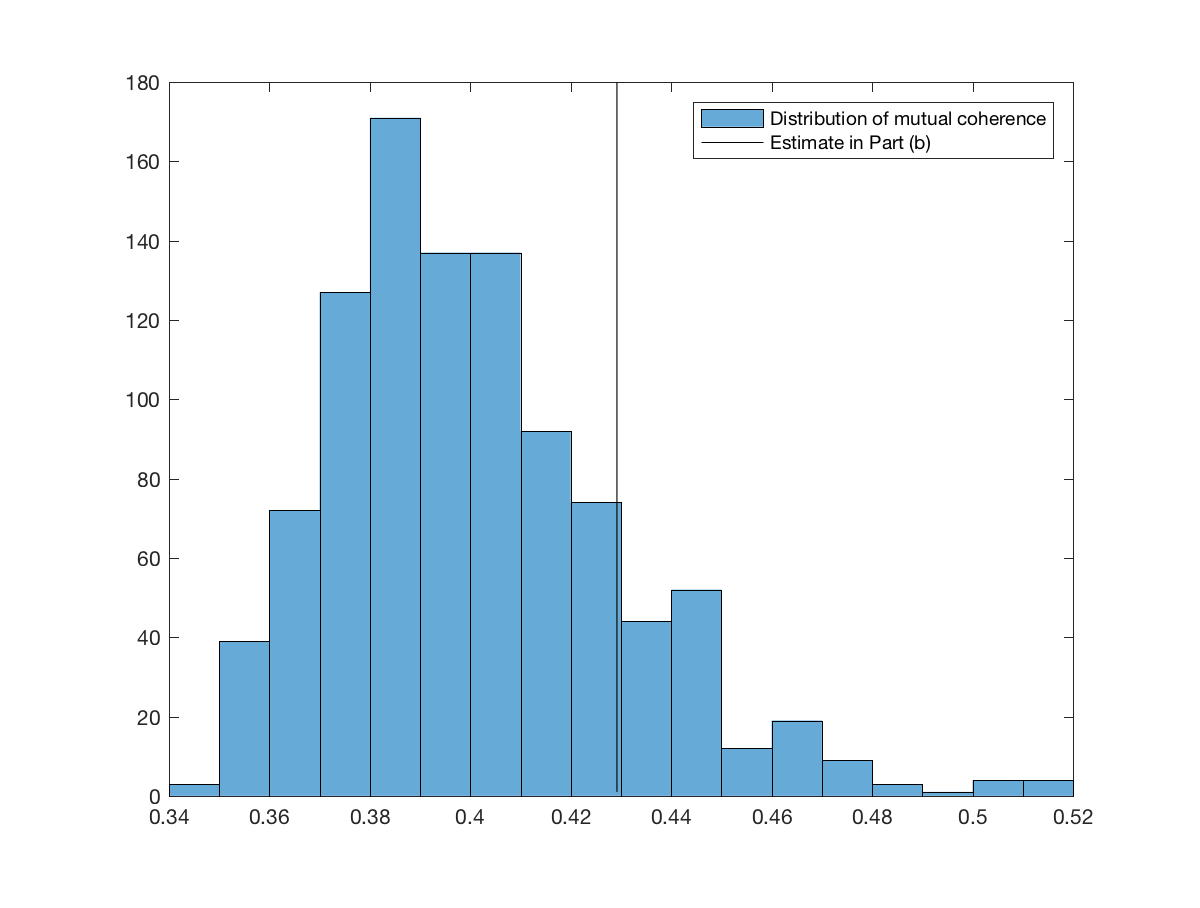
\includegraphics[width=0.6\columnwidth]{./figures/histo.eps}\\
  \caption{Empirical distribution of the mutual coherence.}
  \label{fig:emp}
\end{figure}

}


\newpart{0}
We now generalize the mutual coherence measure to accommodate a more general set of vectors beyond two bases. Specifically, for any given matrix $\bm{A} = [\bm{a}_1, \cdots, \bm{a}_p] \in \mathbb{R}^{n\times p}$ obeying $n \leq  p$, define the mutual coherence of $\bm{A}$ as
\[
  \mu(\bm{A} ) = \max_{1\leq i,j\leq p, ~i\neq j} \left| \frac{\bm{a}_i^{\top} \bm{a}_j}{ \| \bm{a}_i \| \| \bm{a}_j \|  }  \right|.
\]

Show that
\[
  \mu(\bm{A})\geq\sqrt{\frac{p-n}{p-1}\cdot\frac{1}{n}}.
\]
This is a special case of the Welch bound.

\vspace{0.5em}
Hint: you may want to use the following inequality: for any positive semidefinite $\bm{M}\in \mathbb{R}^{n\times n}$,  $\| \bm{M} \|_{\mathrm{F}}^2 \geq \frac{1}{n} \left( \sum_{i=1}^n \lambda_i(\bm{M}) \right)^2$. 

\solution{ Without loss of generality, it is assumed that $\| \bm{a}_i\| =1$ for all $1\leq i \leq p$. To begin with, we find it convenient to work with the Gram matrix  $\bm{A}^{\top}\bm{A}$, since the $(i,j)$ entry of $\bm{A}^{\top}\bm{A}$ is exactly $\bm{a}_i^{\top} \bm{a}_j$. It is seen that
\begin{eqnarray}
  \sum_{1\leq i,j\leq p} \left(\bm{a}_{i}^{\top}\bm{a}_{j}\right)^{2} 
  & = & \left\Vert \bm{A}^{\top}\bm{A}\right\Vert _{\mathrm{F}}^{2}
    =  \sum_{i=1}^{n} \lambda_{i}^2 \left(\bm{A}^{\top}\bm{A}\right)\\
  & \geq & \frac{1}{n} \left(\sum_{i=1}^{n}\lambda_{i} \left(\bm{A}^{\top}\bm{A}\right)\right)^2 \label{eq:Cauchy-Schwarz} \\
  & = & \frac{1}{n} \left(\mathrm{Tr}\left(\bm{A}^{\top}\bm{A}\right)\right)^{2}
    = \frac{p^{2}}{n},
\end{eqnarray}
where (\ref{eq:Cauchy-Schwarz}) follows from the elementary inequality $\frac{1}{n}\sum_{i=1}^n x_i \leq \sqrt{ \frac{1}{n}\sum_{i=1}^n x_i^2 }$ (an immediate consequence of the Cauchy-Schwarz inequality). 

On the other hand, we can connect $\sum_{1\leq i,j\leq p}\left(\bm{a}_{i}^{\top}\bm{a}_{j}\right)^{2}$ with the mutual coherence measure as follows
\begin{eqnarray*}
\sum_{1\leq i,j\leq p}\left(\bm{a}_{i}^{\top}\bm{a}_{j}\right)^{2} & = & \sum_{1\leq i\leq p}\left(\bm{a}_{i}^{\top}\bm{a}_{i}\right)^{2}+\sum_{1\leq i,j\leq p,\text{ }i\neq j}\left(\bm{a}_{i}^{\top}\bm{a}_{j}\right)^{2}\\
 & = & p+\sum_{1\leq i,j\leq p,\text{ }i\neq j}\left(\bm{a}_{i}^{\top}\bm{a}_{j}\right)^{2}\\
 & \leq & p + p(p-1) \mu^2(\bm{A}).
\end{eqnarray*}

Putting the above two bounds together yields 
\[
  p + p(p-1) \mu^2(\bm{A}) \geq \frac{p^{2}}{n},
\]
which immediately establishes the claim.
}


\end{problem}


%\begin{problem}{Picket-fence signal}{10}
%
%Suppose that $\sqrt{n}$ is an integer. Let $\bm{x} \in \mathbb{R}^n$ be a  picket-fence signal with uniform spacing $\sqrt{n}$ such that
%\[
%   x_i = \begin{cases} 1, \quad & \text{if } \frac{i-1}{\sqrt{n}} \text{ is an integer}, \\ 0, & \text{else}, \end{cases} \qquad i = 1,\cdots, n.
%\]
%Compute
%\[
%  \| \bm{x} \|_0 \cdot \| \bm{F} \bm{x} \|_0  \quad \text{and}\quad \| \bm{x} \|_0 + \| \bm{F} \bm{x} \|_0 ,
%\]
%where $\bm{F}$ is the Fourier matrix such that
%\[
%  (\bm{F})_{k,l} = \frac{1}{\sqrt{n}} \exp\left( - i\frac{2\pi (k-1)(l-1)}{n} \right),  \qquad 1\leq k,l \leq n.
%\]
%
%How do they compare to the uncertainty principles we derive in class?
%
%%{\bf Remark:} since $\mu(\bm{I}, \bm{F}) = \frac{1}{\sqrt{n}}$, this justisfies the tightness of our uncertainty principle  $\| \bm{x} \|_0 \cdot \| \bm{F} \bm{x} \|_0 \geq 1 / \mu^2(\bm{I}, \bm{F})$ and $\| \bm{x} \|_0 + \| \bm{F} \bm{x} \|_0 \geq 2 / \mu(\bm{I}, \bm{F})$. 
%
%
%\solution{
%It is easy to verify that
%\[
%  \bm{F} \bm{x} = \bm{x}.
%\]
%To see this, note that the $j$-th element of $\bm{F}\bm{x}$ is
%	\begin{align}
%	[\bm{F}\bm{x}]_j	&=\sum_{m=1}^n \frac{1}{\sqrt{n}}\exp\left(-i\frac{2\pi(j-1)(m-1)}{n}\right) x_m\\
%	&=\sum_{k=0}^{\sqrt{n}-1} \frac{1}{\sqrt{n}}\exp\left(-\frac{2\pi(j-1)\sqrt{n}k}{n}\right),\label{eqn:def}
%	\end{align}
%where \eqref{eqn:def} follows because $x_i$ is 1 when $i-1$ is an integer multiple of $\sqrt{n}$, and is zero otherwise.
%If $j-1$ is an integer multiple of $\sqrt{n}$, then 
%	\begin{align*}
%	\exp\left(-i\frac{2\pi(j-1)}{\sqrt{n}}\right)=1,	
%	\end{align*}
%and therefore, $[\bm{F}\bm{x}]_j$ becomes
%	\begin{align*}
%	[\bm{F}\bm{x}]_j&=\frac{1}{\sqrt{n}}\sum_{k=0}^{\sqrt{n}-1} 	1^k=1.
%	\end{align*}
%If $j-1$ is not an integer multiple of $\sqrt{n}$, then 
%	\begin{align*}
%	[\bm{F}\bm{x}]_j&=\frac{1}{\sqrt{n}}\sum_{k=0}^{\sqrt{n}-1} \left[\exp\left(-\frac{2\pi(j-1)}{\sqrt{n}}\right)\right]^k=\frac{1}{\sqrt{n}}\frac{\exp\left(-i2\pi(j-1)\right)-1}{\exp\left(-i\frac{2\pi(j-1)}{\sqrt{n}}\right)-1}=0.
%	\end{align*}
%Hence,	
%	\begin{align*}
%	[\bm{F}\bm{x}]_j&=\left\lbrace\begin{array}{ll} 1,&\text{if }\frac{j-1}{\sqrt{n}}\text{ is an integer},\\0,&\text{otherwise,}	\end{array}\right.
%	\end{align*}
%or equivalently, $\bm{F}\bm{x} = \bm{x}$.
%
%As a result, $\| \bm{x} \|_0 = \| \bm{F} \bm{x} \|_0 = \sqrt{n}$, and hence $\| \bm{x} \|_0 \cdot \| \bm{F} \bm{x} \|_0  = n$ and $\| \bm{x} \|_0 + \| \bm{F} \bm{x} \|_0  = 2\sqrt{n}$. Since $\mu(\bm{I}, \bm{F}) = \frac{1}{\sqrt{n}}$, this justisfies the tightness of our uncertainty principles  $\| \bm{x} \|_0 \cdot \| \bm{F} \bm{x} \|_0 \geq 1 / \mu^2(\bm{I}, \bm{F})$ and $\| \bm{x} \|_0 + \| \bm{F} \bm{x} \|_0 \geq 2 / \mu(\bm{I}, \bm{F})$.
%}
%
%\end{problem}
%

\begin{problem}{$\ell_1$ minimization}{30}

Suppose that $\bm{A}$ is an $n \times 2n$ dimensional matrix. Let $\bm{x} \in \mathbb{R}^{2n}$ be an unknown $k$-sparse vector, and $\bm{y} = \bm{A}\bm{x}$  the observed system output. This problem is concerned with $\ell_1$ minimization (or basis pursuit) in recovering $\bm{x}$, i.e.   
\begin{equation}
  \text{minimize}_{\bm{z} \in \mathbb{R}^{2n}} ~~\| {\bm{z}} \|_1  \quad \text{s.t. } \bm{A} \bm{z} = \bm{y}.  \label{eq:L1}
\end{equation}


\newpart{0} An optimization problem is called a linear program (LP) if it has the form
\begin{eqnarray*}
\text{minimize}_{\bm{z}} &  & \bm{c}^{\top}\bm{z}+\bm{d}\\
\text{s.t.} &  & \bm{G}\bm{z}\leq\bm{h}\\
 &  & \bm{A}\bm{z}=\bm{b}
\end{eqnarray*}
where $\bm{c},\bm{d},\bm{G},\bm{h},\bm{A}$, and $\bm{b}$ are known. Here, for any two vectors $\bm{r}$ and $\bm{s}$, we say $\bm{r} \leq \bm{s}$ if $r_i \leq s_i$ for all $i$.  Show that (\ref{eq:L1}) can be converted to a linear program. 


\solution{
The given problem is
	\begin{align}
	\mathrm{minimize}_{\bm{z}\in\mathbb{R}^{2n}} \|\bm{z}\|_1\quad \mathrm{s.t.}\quad\bm{A}\bm{z}=\bm{y}.	\label{eqn:l1}
	\end{align}
This can be converted to 
	\begin{align}
	\mathrm{minimize}_{\bm{z}\in\mathbb{R}^{2n},\bm{s}\in\mathbb{R}^{2n}} \bm{1}^T\bm{s} \quad\mathrm{s.t.}\quad \bm{A}\bm{z}=\bm{y}, ~|z_i|\leq s_i~\forall~i.\label{eqn:linear}	
	\end{align}
Denote optimal solutions achieving two problems as $\hat{\bm{z}}$ and $\bar{\bm{z}},\bar{\bm{s}}$, respectively.
Then, 
	\begin{align*}
	\|\hat{\bm{z}}\|_1\stackrel{(a)}{\leq }\|\bar{\bm{z}}\|_1\stackrel{(b)}{\leq}  \bm{1}^T\bar{\bm{s}},	
	\end{align*}
where $(a)$ holds because $\hat{\bm{z}}$ is minimizing the L1 norm, and $(b)$ holds because of the feasibility condition of \eqref{eqn:linear}.
Furthermore, we can prove that
	\begin{align*}
	\|\hat{\bm{z}}\|_1\geq \bm{1}^T\bar{\bm{s}}.	
	\end{align*}
Take solution of \eqref{eqn:linear} as $z_i=\hat{z}_i$ and $s_i=|z_i|$. Then, these vectors are feasible, and the objective value becomes $\|\hat{\bm{z}}\|$. Thus, the objective value of $\bar{\bm{s}}$, which is an optimal solution, should be lower than or equal to $\|\hat{\bm{z}}\|$.

It was shown that 
	\begin{align*}
		\|\hat{\bm{z}}\|_1=\bm{1}^{\top}\bm{\bar{\bm{s}}},
	\end{align*}
which implies that the problem \eqref{eqn:l1} can be converted to \eqref{eqn:linear}. 
The problem \eqref{eqn:linear} can be rewitten as
	\begin{align*}
	\mathrm{minimize}_{\bm{z}\in\mathbb{R}^{2n},\bm{s}\in\mathbb{R}^{2n}} \bm{1}^T\bm{s} \quad\mathrm{s.t.}\quad \bm{A}\bm{z}=\bm{y}, ~\bm{z}-\bm{s}\leq\bm{0},~-\bm{z}-\bm{s}\leq 0	,
	\end{align*}
which is a linear program.
}




\newpart{0} 
	Set $n=256$, and let $k$ range between 1 and 128.  For each choice of $k$, run 10 independent numerical experiments: in each experiment, generate $\bm{A} = [a_{i,j}]_{1\leq i\leq n, 1\leq j\leq 2n}$ as a random matrix such that the $a_{i,j}$'s are i.i.d.~standard Gaussian random variables,  generate $\bm{x} \in \mathbb{R}^{2n}$ as a random $k$-sparse signal (e.g.~you may generate the support of $\bm{x}$ uniformly at random, with each non-zero entry drawn from the standard Gaussian distribution),  and solve (\ref{eq:L1}) with $\bm{y} = \bm{A}\bm{x}$.  An experiment is claimed successful if the solution $\bm{z}$ returned by (\ref{eq:L1}) obeys $\| \bm{x} - \bm{z} \|_2 \leq 0.001 \| \bm{x} \|_2$. 
Report the empirical success rates (averaged over 10 experiments) for each choice of $k$. 
\end{problem}

\solution{
The support of $\bm{x}$ can be randomly chosen by using MATLAB built-in function randperm.
Using cvx program, $\bm{z}$ can be computed, where feasibility conditions are arranged as
	\begin{align*}
	&\bm{A}\bm{z}=\bm{y},\\
	&\left[\begin{array}{ll}\bm{I}&-\bm{I}\end{array}\right]\left[\begin{array}{l} \bm{z}\\\bm{s}	\end{array}\right]\leq \bm{0},\\
	&\left[\begin{array}{ll}-\bm{I}&-\bm{I}\end{array}\right]\left[\begin{array}{l} \bm{z}\\\bm{s}	\end{array}\right]\leq \bm{0}.
	\end{align*}
Success rate for each $k$ is given in Fig. \ref{fig:success}
\begin{figure}[ht]
\centering
  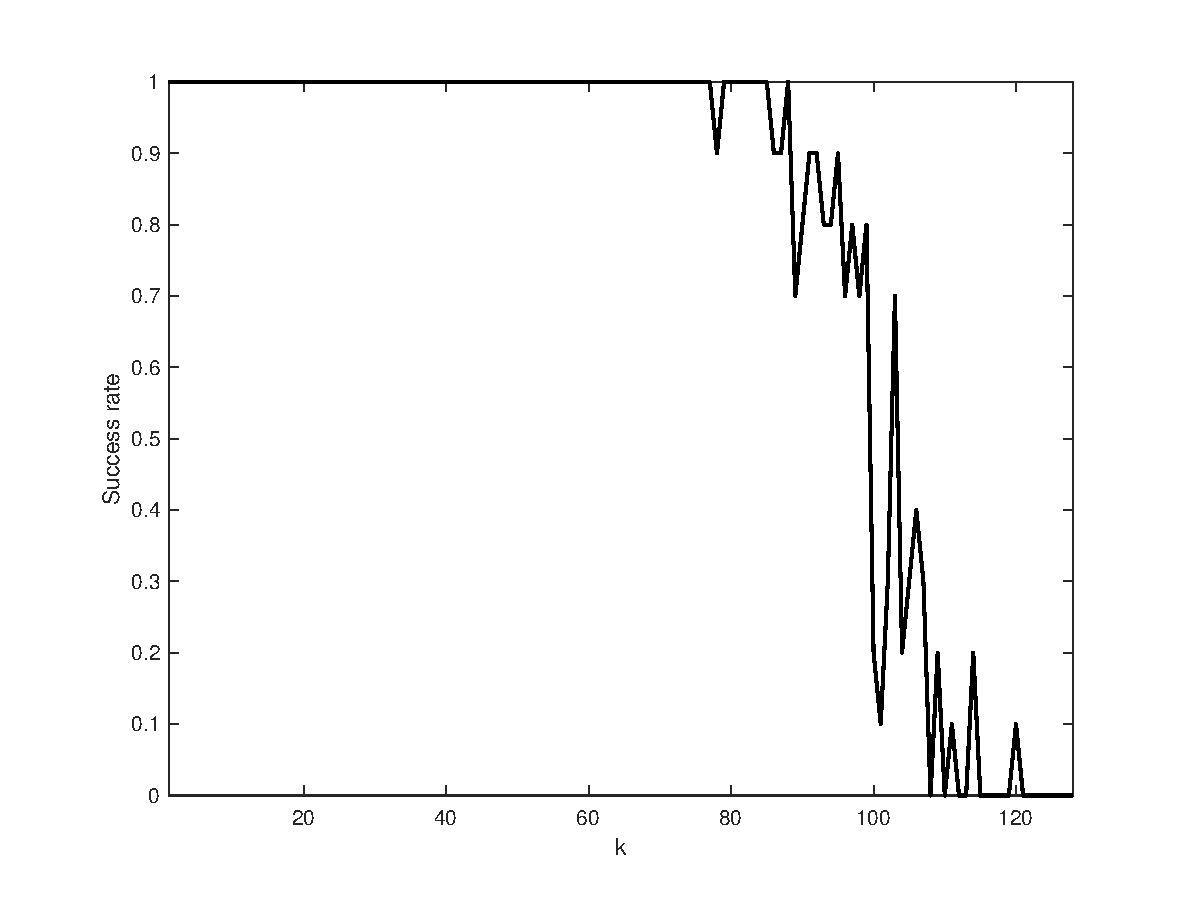
\includegraphics[width=0.6\columnwidth]{./figures/success.eps}\\
  \caption{Success rate for each $k\in\{1,\cdots,128\}$ with 10 expriments.}
  \label{fig:success}
\end{figure}
This graph shows that success rate is higher for sparse signals.
}




%%%%%%%%%%%%%%%%%%%%%%%%%%%%%%%%%%%%%%%%%%%%%%%%%%%%%%%%%%%%
\begin{problem}{Restricted isometry properties}{30}

Recall that the restricted isometry constant $\delta_s \geq 0$ of 
$\bm{A}$ is the smallest constant such that 
\begin{equation}
  \label{eq:defn-RIP}
  (1-\delta_{s}) \| \bm{x} \|_2^2 \leq \|\bm{A} \bm{x}  \|_2^2 \leq  (1+\delta_{s}) \| \bm{x} \|_2^2
\end{equation}
holds for all $s$-sparse vector $\bm{x} \in \mathbb{R}^p$.

\newpart{0} Show that
$$|\langle \bm{A} \bm{x}_1, \bm{A} \bm{x}_2 \rangle | \leq \delta_{s_1+s_2} \| \bm{x}_1\|_2\|\bm{x}_2\|_2$$
for all pairs of $\bm{x}_1$ and $\bm{x}_2$ that are supported on disjoint subsets $S_1, S_2\subset \{1,\cdots,n\}$ with $|S_1|\leq s_1$ and $|S_2|\leq s_2$.

\solution{
WLOG, assume $\|\bm{x}_1\|=\|\bm{x}_2\|=1$. Since $\bm{x}_1$ and $\bm{x}_2$ have disjoint support, we get
\begin{align*}
| \langle \bm{A} \bm{x}_1, \bm{A}\bm{x}_2 \rangle | 
&  = \frac{1}{4} \left| \| \bm{A}\bm{x}_1 + \bm{A}\bm{x}_2\|_2^2 - \| \bm{A}\bm{x}_1 - \bm{A}\bm{x}_2\|_2^2 \right| \\
&  = \frac{1}{4}\left|\left\Vert \bm{A}\left[\begin{array}{c}
\bm{x}_{1}\\
\bm{x}_{2}
\end{array}\right]\right\Vert ^{2}-\left\Vert \bm{A}\left[\begin{array}{c}
\bm{x}_{1}\\
-\bm{x}_{2}
\end{array}\right]\right\Vert ^{2}\right| \\
& \leq  \frac{1}{4} |2(1+\delta_{s_1+s_2}) -2(1- \delta_{s_1+s_2}) | \\
& \leq \delta_{s_1+s_2}.
\end{align*}

}

\newpart{0} For any $\bm{u}$ and $\bm{v}$, show that
\[
|\langle\bm{u},\text{ }(\bm{I}-\bm{A}^{\top}\bm{A})\bm{v}\rangle|\leq\delta_{s}\|\bm{u}\|_2 \cdot\|\bm{v}\|_2,
\]
where $s$ is the cardinality of $\text{support}\left(\bm{u}\right) \cup\text{support}\left(\bm{v}\right)$. 

\solution{
%Yeohee, you can take a look at Lemma 6.16 of \url{http://human-robot.sysu.edu.cn/ebook/preprint093.pdf}
Let $\mathcal{S}=\text{support}\left(\bm{u}\right) \cup\text{support}\left(\bm{v}\right)$.
	\begin{align*}
	|\langle\bm{u},(\bm{I}-\bm{A}^{\top}\bm{A})\bm{v}\rangle|&=|\langle\bm{u},\bm{v}\rangle-\langle\bm{A}\bm{u},\bm{A}\bm{v}\rangle|\\
	&=|\langle\bm{u}_{\mathcal{S}},\bm{v}_{\mathcal{S}}\rangle-\langle\bm{A}_{\mathcal{S}}\bm{u}_{\mathcal{S}},\bm{A}_{\mathcal{S}}\bm{v}_{\mathcal{S}}\rangle|\\
	&=|\langle \bm{u}_{\mathcal{S}},(\bm{I}-\bm{A}_{\mathcal{S}}^{\top}\bm{A}_{\mathcal{S}})\bm{v}_{\mathcal{S}}\rangle|\\
	&\leq \|\bm{u}_{\mathcal{S}}\|_2 \|\bm{I}-\bm{A}_{\mathcal{S}}^{\top}\bm{A}_{\mathcal{S}}\|_{\mathsf{op}} \|\bm{v}_{\mathcal{S}}\|_2,
	\end{align*}
where $\|\cdot\|_{\mathsf{op}}$ denotes the operator norm of a matrix as
	\begin{align*}
	\|\bm{A}\|_{\mathsf{op}}=\max_{\|\bm{x}\|_2=1} \|\bm{A}\bm{x}\|_2.
	\end{align*}
By the definition of the restricted isometry constant,
	\begin{align*}
	|\langle (\bm{A}_{\mathcal{S}}^{\top}\bm{A}_{\mathcal{S}}-\bm{I})\bm{x},\bm{x}\rangle|=|\langle\bm{A}_{\mathcal{S}}\bm{x},\bm{A}_{\mathcal{S}}\bm{x}\rangle-\langle\bm{x},\bm{x}\rangle|=| \|\bm{A}_{\mathcal{S}}\bm{x}\|^2-\|\bm{x}\|_2^2|\leq \delta_s \|\bm{x}\|_2^2.
	\end{align*}
Therefore,	
	\begin{align*}
	\|\bm{I}-\bm{A}_{\mathcal{S}}^{\top}\bm{A}_{\mathcal{S}}\|_{\mathsf{op}}	\leq \delta_s
	\end{align*}
and
	\begin{align*}
	|\langle\bm{u},(\bm{I}-\bm{A}^{\top}\bm{A})\bm{v}\rangle|\leq\delta_s \|\bm{u}_{\mathcal{S}}\|_2 \|\bm{v}_{\mathcal{S}}\|_2	=\delta_s \|\bm{u}\|_2\|\bm{v}\|_2.
	\end{align*}




}


\newpart{0} Suppose that each column of $\bm{A}$ has unit norm.  Show that $\delta_2 = \mu(\bm{A})$, where $\mu(\bm{A})$ is the mutual coherence of $\bm{A}$. 

\solution{Given that 
	\begin{align*}
	|\langle (\bm{A}_{\mathcal{S}}^{\top}\bm{A}_{\mathcal{S}}-\bm{I})\bm{x},\bm{x}\rangle|=|\langle\bm{A}_{\mathcal{S}}\bm{x},\bm{A}_{\mathcal{S}}\bm{x}\rangle-\langle\bm{x},\bm{x}\rangle|=| \|\bm{A}_{\mathcal{S}}\bm{x}\|^2-\|\bm{x}\|^2|\leq \delta_s \|\bm{x}\|^2,
	\end{align*}
$\delta_s$ is the same as
	\begin{align*}
	\delta_s=\max_{|\mathcal{S}|\leq s} \|\bm{A}_{\mathcal{S}}^{\top}\bm{A}_{\mathcal{S}}-\bm{I}\|_{\mathsf{op}}.
	\end{align*}
When $s=2$,
	\begin{align*}
	\delta_2=\max_{i\neq j} \left\| \left[\begin{array}{ll}\bm{a}_i&\bm{a}_j\end{array}\right]	^{\top}\left[\begin{array}{ll}\bm{a}_i&\bm{a}_j\end{array}\right]-\bm{I}\right\|_{\mathsf{op}}.
	\end{align*}
The eigenvalues of the following matrix
	\begin{align*}
	 \left[\begin{array}{ll}\bm{a}_i&\bm{a}_j\end{array}\right]	^{\top}\left[\begin{array}{ll}\bm{a}_i&\bm{a}_j\end{array}\right]-\bm{I}=\left[\begin{array}{ll} 1 & \langle \bm{a}_i,\bm{a}_j\rangle \\ \langle \bm{a}_i,\bm{a}_j\rangle  & 1\end{array}\right]-\bm{I}=	\left[\begin{array}{ll} 0 & \langle \bm{a}_i,\bm{a}_j\rangle \\ \langle \bm{a}_i,\bm{a}_j\rangle  & 0\end{array}\right]	
	\end{align*}
	are $\pm \langle \bm{a}_i,\bm{a}_j\rangle$, and accordingly
	\begin{align*}
	\delta_2=\max_{i\neq j} |\langle \bm{a}_i,\bm{a}_j\rangle| =\mu(\bm{A}).
	\end{align*}

	
}

\end{problem}



\end{document}
